\documentclass[handout]{beamer}
\usetheme{CambridgeUS} % replace it with Boadilla if you want no section bar
%\usecolortheme{crane} % other ones: dove, dolphin, rose, seahorse, orchid, crane, seagull, lily, wolverine
%\usefonttheme{serif} 
\usefonttheme[onlymath]{serif} % uncomment if you want it just for math

\setbeamertemplate{navigation symbols}{}  % comment to have nagivation

\usepackage[compress,comma,authoryear]{natbib}
\usepackage{tikz}
\usetikzlibrary{mindmap,trees}
\usepackage{amsmath,mathtools}
\usepackage{amsthm}
\usepackage{booktabs}
\usepackage{graphicx,epstopdf}
\usepackage{hyperref}


\definecolor{blue}{RGB}{0,114,178}
\definecolor{orange}{RGB}{213,94,0}
\definecolor{red}{RGB}{190,0,0}
\definecolor{yellow}{RGB}{240,228,66}
\definecolor{green}{RGB}{0,158,115}
\definecolor{Lblue}{RGB}{0,197,155}
\definecolor{Dblue}{RGB}{0,76,119}
\definecolor{Lgreen}{RGB}{180,255,230}

\hypersetup{
	colorlinks=false,
	linkbordercolor = {white},
	linkcolor = {blue}
}
\definecolor{MyBackground}{RGB}{245,245,245}

\setbeamercolor{frametitle}{fg=blue}
\setbeamercolor{title}{fg=blue}
\setbeamertemplate{footline}[frame number]
\setbeamertemplate{navigation symbols}{} 
\setbeamertemplate{itemize item}[circle]%{$\bigstar$}
\setbeamertemplate{itemize subitem}{$\bigstar$}
\setbeamercolor{itemize item}{fg=blue}
\setbeamercolor{itemize subitem}{fg=blue}
\setbeamercolor{enumerate item}{fg=blue}
\setbeamercolor{enumerate subitem}{fg=blue}
\setbeamercolor{button}{bg=MyBackground,fg=blue}
\setbeamercolor*{palette primary}{use=structure,fg=blue,bg=white}
\setbeamercolor*{palette secondary}{use=structure,fg=white,bg=Dblue}
\setbeamercolor*{palette tertiary}{use=structure,fg=white,bg=blue}
\setbeamercolor*{palette quaternary}{fg=white,bg=black}
\setbeamercolor*{palettes quaternary}{fg=white,bg=Lgreen}
%\setbeamercolor{titlelike}{parent=structure,bg=Lgreen}
%\setbeamercolor{title in head/foot}{bg=Lgreen,fg=orange}

\setbeamertemplate{enumerate item}{%
	\usebeamercolor[bg]{item projected}%
	\raisebox{1.5pt}{\colorbox{blue}{\color{fg}\footnotesize\insertenumlabel}}%
}



\begin{document}
	\title[Econometrics 2]{Econometrics 2 (M.Sc.)}
	\subtitle{Matching}
	\author[Mohammad Hoseini]{Mohammad Hoseini}
	
	%\institute[IMPS]{Institute for Management and Planning Studies (IMPS)}
	
	\date[Spring 2024]{Spring 2024 \\
	\vspace{10pt} @metrics2
}
	
\begin{frame}[plain]
	\titlepage
\end{frame}

\section{Matching}
\subsection{Introduction}

\begin{frame}{Motivation}
In the previous lecture, we saw when CIA holds, how we can use regression to estimate treatment effect \textit{ conditional on observables:} $E[Y_i^1-Y_i^0 |X_i]$\bigskip

In this lecture, we discuss another method to remove selection bias when CIA holds.\bigskip

This method is called \textbf{matching}, which is a nonparametric way of controlling for $X$.\bigskip	

Its basic idea is to use observables to match similar units in different groups and estimate the treatment effect by averaging the effects between similar units.\bigskip

Note that all we said about what $X$ to control in regression (common factors vs. bad controls) are valid for matching too.
	
\end{frame}


\begin{frame}{Matching}
	\[\text{Observed effect: } E[Y_i|D_i=1]-E[Y_i|D_i=0]=\frac{1}{N_T}\sum_{i\in T}Y_i-\frac{1}{N_C}\sum_{i\in C}Y_i \]
	When treatment (T) and control (C) groups differ in observed covariates $X$, we have selection bias.\bigskip
	
	If CIA holds, we can estimate treatment effect by \textit{'matching'} each unit in treatment (control) group with similar units in control (treatment) and comparing Y between them:\medskip
	
	\begin{itemize}
		\item For each unit $i \in T$, we find its pair $j \in C$, such that $X_i\approx X_j$.
		\item Let $j=C(i)$ be the matched control unit for the treated unit $i$, then we can compute treatment effect on the treated units as
	\end{itemize}
	\[\frac{1}{N_T}\sum_{i\in T}Y_i-Y_{C(i)}\]   
	
\end{frame}

\begin{frame}{Different steps to estimate effect with matching}
	\begin{enumerate}
		\item Choosing variables $X$ for matching units
		\begin{itemize}
			\item Same logic as for regression: include pre treatment variables, but not post treatment.
		\end{itemize}\bigskip
	
	\item Determine the values of $X$ for matching.
		\begin{itemize}
			\item It is quite possible that treatment and control group does not overlap on some values of $X$.
			\item For these values, we cannot perform matching (support problem)
		\end{itemize}\bigskip
	
	\item Choosing matching method to construct the matched sample.\bigskip
	 
	\item Using a matching estimator to estimate the treatment effect using the matched sample.
	\end{enumerate}
\end{frame}

\subsection{Matching methods}

\begin{frame}{Support problem}
	Support problem: the value of $X$ observed for the treatment group may not overlap much with the control group.	
	For example, most treated subjects have $X=x_1$ while most controls have $X=x_0$.\bigskip
	
	Suppose we have 3 treated ($T_1, T_2, T_3$) and 4 control ($C_1, C_2, C_3, C_4$) units that are matched as follows:
	\begin{itemize}
		\item $T_1: C_1, C_2$
		\item $T_2: C_4$
		\item $T_3:$ no matched control
	\end{itemize}

There are two successfully matched treated. As $T_3$ has no good match, we drop it from matching. In the original sample, there was 7 observations, but in the matched sample 5 observations.
\end{frame}

\begin{frame}{Matching details}
	To implement matching, we have to choose between a number of options in different dimensions:
	\begin{itemize}
		\item How the measure distance for matching?
		\begin{itemize}
			\item Exact matching
			\item Mahalanobis distance matching
			\item Propensity score matching
		\end{itemize}
		\item Match based on an interval for matching or a fixed number of matched?
		\begin{itemize}
			\item Caliper matching
			\item Nearest neighbor matching
		\end{itemize}
		\item Pair matching or multi matching?
		\item Match with or without replacement of controls? Is each control matched to at most one treated?
	\end{itemize}
\end{frame}

\begin{frame}{Exact vs. distance matching}
	After selecting the covariate vector $X$, we should determine how to match for each covariate:
	\begin{itemize}
		\item \textbf{Exact matching}: match units if they have exactly the same values. Usually is used for discrete variable with few values such as province, gender, rural/urban, etc.
		\item Distance matching: match units based on a distance measure. There are two main distance measures used in matching
		\begin{itemize}
			\item \textbf{Mahalanobis distance matching}
			\item \textbf{Propensity score matching}
		\end{itemize}
	\end{itemize}\medskip

Most of the time matching is done in two stages. First exact matching (strafication) is done for $X_1$ covariates, and then a distance matching is applied on $X_2$ covariates.\medskip

For instance, in job training example, let $X_1$=(gender, age group), and $X_2$=(schooling years, job experience). In this way, we make sure that all males/females and young/old people are matched with the same gender and age groups.
\end{frame}


\begin{frame}{Nearest neighbor and caliper matching}
	
We should also decide whether to match based on number, interval, or a combination of both:\medskip
\begin{itemize}
	\item \textbf{Caliper matching}: all controls within a fixed distance (caliper) to treated are matched.
	\begin{itemize}
		\item Caliper is a `bandwidth' and there is no general rule to determine it. If we have some idea on the absolute value of the desired similarity in $X$, we can choose caliper accordingly.
	\end{itemize}\medskip

	\item \textbf{Nearest neighbour matching}: a fixed number of closest controls are selected irrespective of their distance.
	\begin{itemize}
		\item If only one control (the nearest) is chosen, it is called `pair matching'.
		\item If the number of nearest neighbor $>1$, it is called `multi matching'.
		\item If all treated are matched with at least one control and all controls are matched with at least one treated we have `full matching'.
	\end{itemize} 
	\item Nearest neighbor matching is usually combined with caliper matching to avoid getting very dissimilar matched units.
\end{itemize}
\end{frame}

\begin{frame}{Matching with or without replacement}
	Matching without replacement means that each control unit is matched to at most one treated unit, while matching with replacement means that control units can be reused and matched to multiple treated units.\bigskip 
	
	Matching with replacement will tend to yield better covariate balance, because the problem of ``running out'' of close control units to match to treated units is avoided, but the reuse of control units will decrease the effect sample size, thereby worsening precision. \bigskip
	
	Matching without replacement has some benefits such that weights for each unit can be omitted.
\end{frame}

\begin{frame}{Measuring distance for matching}
	
	{\color{violet} Mahalanobis distance = $(X_T-X_C)'V^{-1}(X_T-X_C)$}, where $V$ is the sample covariance matrix for $X$ (noisy gets lower weight). \bigskip
	
	{\color{teal} Propensity score: $\pi(X)=P(D=1|X)$}, the probability of treatment conditional on $X$.\medskip
	
	Rosenbaum and Rubin (1983) show that if CIA holds ($Y^D\perp D |X$), then  $Y^D\perp D |\pi(X)$.\medskip
	
	This means that propensity score can be used as a balancing score for $X$.\medskip
	
	Estimating the propensity score:
	\begin{itemize}
		\item Estimate $D$ on $X$ using logit, probit, etc. ($D = \alpha_0 +\alpha_1 x_1 +\dots+\alpha_n x_n+\epsilon$)
		\item Obtain the predicted $\pi(X)$ for each unit using above estimation.
	\end{itemize}
\end{frame}

\begin{frame}{Propensity score vs. Mahalanobis distance}
	Dimension problem: If the dimension of $X$ is large, then conditioning on $X$ result in too few observations for each sub population characterized by $X$.\bigskip
	
	Using propensity score $\pi(X)$ instead of $X$ in conditioning is a considerable reduction of dimension 	because $\pi(X)$ is one-dimensional.\bigskip
	
	Mahalanobis distance is less effective when covariate balance is good for many elements in $X$.	
	In fact, balanced variables become insignificant in estimating $\pi(X)$, but they get weight in Mahalanobis distance. We want to balance the unbalanced variables.\bigskip
	
	$\pi(X)$ more is convenient for presentation, as it is one dimensional and lies between 0 and 1.
	
	
\end{frame}

\begin{frame}{Mahalanobis distance vs. propensity score}

	Mahalanobis distance has good robustness property and unlike $\pi(X)$ is not vulnerable to a misspecified model for estimating $D$ on $X$.\bigskip 
	
	Mahalanobis distance better balances the covariates when the control sample is large enough.\bigskip
	
	Mahalanobis usually works better than PS when $D$ is not a endogenous treatment and you want to build two similar populations based on a list of variables (Iran vs. Afghan workers). 
	
\end{frame}


\subsection{Matching estimators}
\begin{frame}{Effect on treated, control, and whole population}
Conditional treatment effects on:
\begin{itemize}
	\item the treated: $\delta_1(X)=E[Y^1_i-Y^0_i|X_i,D_i=1]$
	\item the untreated: $\delta_0(X)=E[Y^1_i-Y^0_i|X_i,D_i=0]$	
	\item whole population: $\delta(X)=E[Y^1_i-Y^0_i|X_i]=\delta_0(X)P(D=0|X)+\delta_1(X)P(D=1|X)$	
\end{itemize} \pause \bigskip

Let $f(x)$ be the density function of distribution of $X$.\medskip

Then, `unconditional' treatment effects on the:
\begin{itemize}
	\item treated: $\delta_1=E[Y^1_i-Y^0_i|D_i=1]=E\big[E[Y^1_i-Y^0_i|X_i,D_i=1]\big]=\int_{x|D=1} \delta_1(x)f(x)dx$
	\item untreated: $\delta_0=E[Y^1_i-Y^0_i|D_i=0]=E\big[E[Y^1_i-Y^0_i|X_i,D_i=0]\big]=\int_{x|D=0} \delta_0(x)f(x)dx$	
	\item whole population: $\delta=E[Y^1_i-Y^0_i]=\delta_0P(D=0)+\delta_1P(D=1)=\int \delta(x)f(x)dx$	
\end{itemize} 

\end{frame}
 

\begin{frame}{Matching estimator}
	\[\delta_1=E[Y^1_i-Y^0_i|D_i=1] \approx \frac{1}{N_{T_m}}\sum_{i\in{T_m}}\Big[Y_i-\hat{E}[Y|X=X_i,D=0] \Big]\]
	\[\delta_0=E[Y^1_i-Y^0_i|D_i=0] \approx \frac{1}{N_{C_m}}\sum_{j\in{C_m}}\Big[\hat{E}[Y|X=X_j,D=1]-Y_j \Big]\]
	where $T_m$ and $C_m$ are the matchable units in $T$ and $C$ (remember support problem).
	$\hat{E}[Y|X,D]$ is an estimator of $E[Y|X,D]$ that depends on our matching method:
	\begin{itemize}
		\item In pair matching that $i\in T$ is matched to $j\in C$: $\hat{E}[Y|X=X_i,D=0]=Y_{j}$
		\item Multi matching $\hat{E}$: simple average or weighted (distance$^{-1}$) average 
	\end{itemize}
	
	\[\delta=E[Y^1_i-Y^0_i] \approx \frac{1 }{N_{C_m}+N_{T_m}}\Big(N_{C _m} \delta_0 + N_{T_m} \delta_1 \Big) \]
\end{frame}

  
\begin{frame}{Union membership on wage (Vella and Verbeek, 1998)}
Data from the US National Longitudinal Survey for 1987, with $N = 545,\ N_T = 143$\medskip
%Covariates $X$: 
\begin{itemize}
	\item Exact matching on regional dummies (north central, northeast, and south), dummy for rural area, and 12 job industry dummies.
	\item Distance matching on education in years (edu), job experience in years (exr)
\end{itemize}
	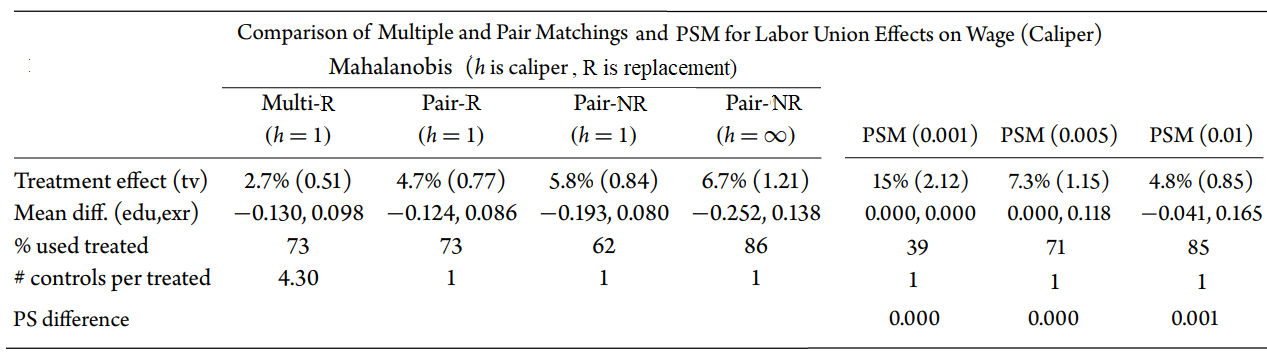
\includegraphics[width=\linewidth]{./Figures/matching2}
\end{frame}

\begin{frame}{Rosenbaum and	Rubin (1985)}
Studying the effects of prenatal exposure to an organic acid on psychological development of Danish children.
T group: 221 exposed children,  C group: 7027 unexposed children.\medskip

\begin{enumerate}
	\item pair propensity score (PS) matching with no caliper
	\item Mahalanobis with no caliper.
	\item PS with caliper and then apply Mahalanobis pair matching among them. If there is no calipered control, then pair PS matching.
\end{enumerate}

Covariate balance check:

	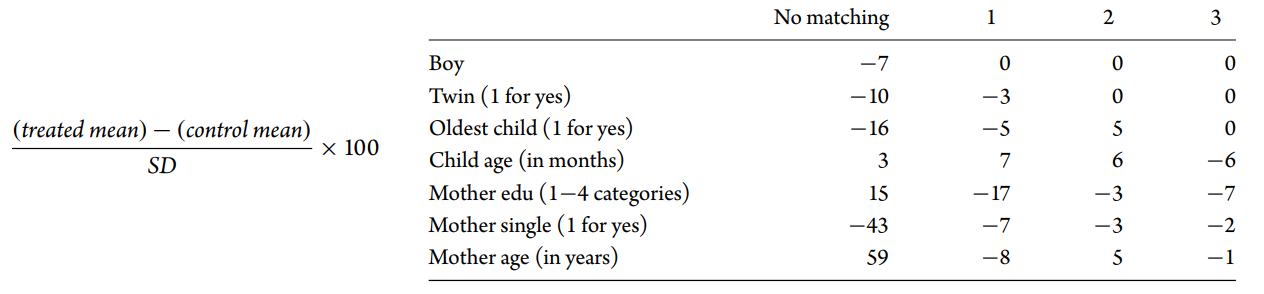
\includegraphics[width=\linewidth]{./Figures/matching1}


\end{frame}

\begin{frame}{Ex-ante program evaluation by matching }
	Effect of welfare program on labor participation (Todd \& Wolpin, 2008) \medskip
	
	A state is going to implement a welfare benefit offered to unmarried women $b(y_i,n_i)$
	\begin{itemize}
		\item $y_i$: nonearned income, $n_i$: number of children, $L_i$: labor participation dummy
	\end{itemize}
Consumption: $\begin{cases} y_i+w_iL_i & \text{w/o benefit}\\ y_i+w_iL_i+b(y_i,n_i)(1-L_i)=\tilde{y_i}+\tilde{w_i}L_i & \text{with  benefit} \end{cases}$\medskip

where $\tilde{y_i}=y_i+b(y_i,n_i)$ and $\tilde{w_i}=w_i-b(y_i,n_i)$\medskip

Before program implementation, we can use this matching estimator
\[\frac{1}{n}\sum_{j=1}^{J} E[L_i|y_i=y_j+b(y_j,n_j),w_i=w_j-b(y_j,n_j)] - L_j(y_j,w_j,n_j)\]
The sample needs to be large enough to find good support for all $j$.
\end{frame}


%\begin{frame}{With inappropriate observables matching goes wrong}
%	\begin{table}
%		\begin{tabular}{|l|c|c|}
%			\hline
%			Observable variables in data& Person 1 & Person 2 \\
%			\hline
%			%occupation & actor & actor \\
%			birth year & 1974 & 1974\\
%			gender & male & male \\
%			marital status & married & married \\
%			children & 1&1\\
%			occupation & actor & actor \\
%			a sample work & Joker & Joker \\
%			\hline
%			&&\\
%			\begin{minipage}{.4\linewidth}
%				{\color{violet}	including unobservables:\vspace*{1.5cm} }
%			\end{minipage}
%			&	
\includegraphics[width=0.15\linewidth]{../figure/Phoniex2}&	
\includegraphics[width=0.15\linewidth]{../figure/ghafourian} \\
%			&Joaquin Phoenix & Mehran Ghafourian \\
%			\hline
%		\end{tabular}
%	\end{table}
%	
%\end{frame}


\begin{frame}{Matching on unobservables}
	So far we discussed matching on the observable variables $X$.\bigskip
	
	Sometimes we can use matching to control for unobservables:
	\begin{itemize}
		\item matching with twins controls for genes.
		\item matching with siblings to control for family effect.
		\item matching with neighbors to control for local effects.
		\item matching with best friend to control for peer pressure.
		\item matching with classmates to control for teacher/school.
		\item $\dots$
	\end{itemize}
\end{frame}



\begin{frame}{The effect of smoking (Freedman 1999)}
Some (smoker) scientists argued that there is a genetic predisposition to smoke and have illnesses. 
In other words, there is a common factor (genes) affecting both smoking and illness occurrences, and thus even
if smoking habit is altered, it will have no effect on illnesses.\bigskip

Freedman (1999) conducted a twin study in Finland by finding 22 identical twin pairs with
each pair consisting of a smoker and a nonsmoker\pause
\begin{columns}
	\begin{column}{0.99\textwidth}
		\begin{itemize}
			\item the smoker died first in 17 pairs for all causes,
			\item in 9 pairs only one twin died of a heart disease, those 9 were all smokers!
			\item in 2 pairs only one twin died of lung cancer, those 2 were all smokers!
		\end{itemize}
	\end{column}
%\begin{column}{0.2\textwidth}
%	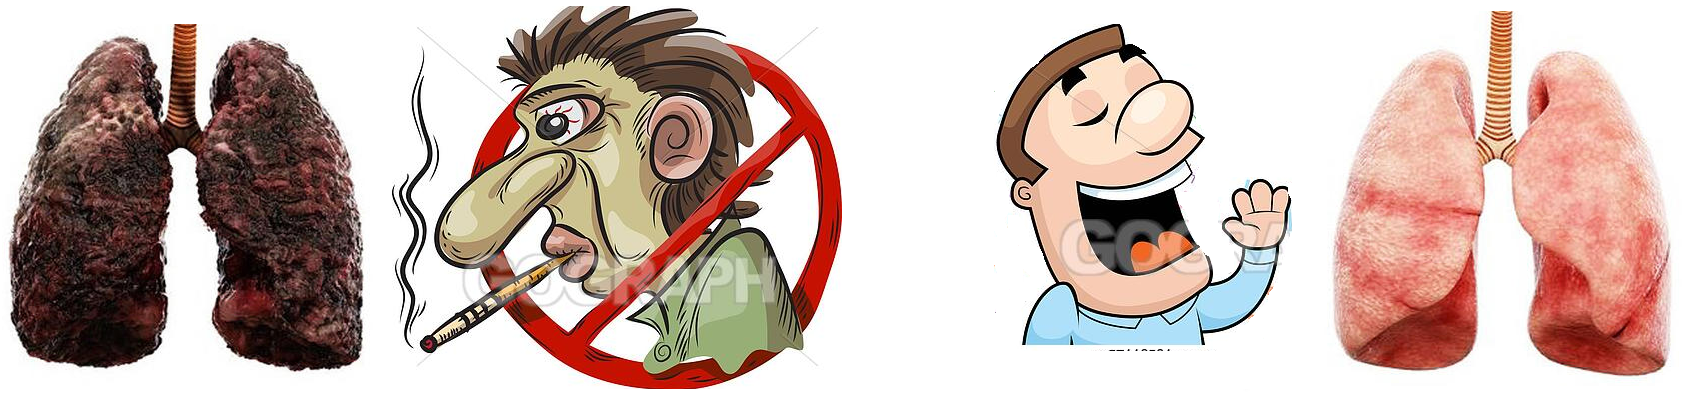
\includegraphics[width=.8\textwidth]{./Figures/smoking.png}
%\end{column}
\end{columns}


\end{frame}

\begin{frame}{Matching vs. Regression}
When CIA holds, we can use regression to estimate treatment effect \textit{\color{magenta} conditional on observables:} $E[Y_i^1-Y_i^0{\color{magenta} |X_i}]$\bigskip

Although CIA with regression eliminate selection bias, what can we say about \textit{\color{teal} unconditional treatment effect}, $E[Y_i^1-Y_i^0]$, when CIA holds?\pause\medskip

Remember: ${\color{magenta} E\Big[ } E[Y_i^1-Y_i^0{\color{magenta} |X_i}]{\color{magenta} \Big]} = E[Y_i^1-Y_i^0]$\medskip

Unconditional treatment effects can be interpreted a weighted average of the conditional treatment effects.\bigskip

Matching estimator estimates unconditional treatment effect. How it is related to regression?
\end{frame}


\begin{frame}{Matching vs. Regression}
CIA: $\delta_x=E[Y_i|X_i=x,D_i=1]-E[Y_i|X_i=x,D_i=0]$ is the conditional treatment effect.\medskip
 
How can we link $\beta_R$ in the saturated regression: $Y_i=\alpha+\beta_R D_i+\sum_x\gamma_x d_{ix} +v_i$ to the matching estimator $\beta_M=E[Y^1_i-Y^0_i|D_i=1]$?\medskip

Angrist and Pishke (2009) show that ($P$ is probability):
 \[\beta_R=\frac{\sum_x \delta_x P(D_i=1|X_i=x)(1-P(D_i=1|X_i=x))P(X_i=x)}{\sum_x P(D_i=1|X_i=x)(1-P(D_i=1|X_i=x))P(X_i=x)} \]
 \[\beta_M=\frac{\sum_x \delta_x P(D_i=1|X_i=x)P(X_i=x)}{\sum_x P(D_i=1|X_i=x)P(X_i=x)} \]
 Both $\beta_R$ and $\beta_m$ are unconditional treatment effects but they are averaged by different weights.
\end{frame}

\begin{frame}{Matching vs. Regression}
$\beta_M$ puts the most weight on covariate cells containing those who are most likely to be treated.\medskip

$\beta_R$  puts the most weight on covariate cells where the conditional variance of treatment status is largest. \begin{itemize}
	\item This variance is maximized when $P(D_i=1|X_i=x)=0.5$, i.e. units where there are equal numbers of treated and control observations.
\end{itemize}\medskip

The difference in weighting schemes of $\beta_M$ and $\beta_R$ is of little importance if $\delta_x$ does not vary much for different values of $x$.\medskip

Support problem: neither $\beta_M$ nor $\beta_R$ give any weight to covariate cells that do not contain both treated and control observations.\medskip

Consider $X_i=x^*$ where either no one is treated or everyone is treated. Then, the regression weights $P(D_i=1|X_i=x^*)(1-P(D_i=1|X_i=x^*))$ is zero and $\delta_{x^*}$ is undefined.
\end{frame}


\end{document}
